\section{Resultados} \label{sec:resultados}
En primer lograr obtendremos lo valores en el visualizador de arduino de la tarjeta IMU sin calibrar \cite{segovia2018adquisicion} que como se observo presentan desvios ya que en el caso del acelerometro los del eje X resultados cercanos a 0.5 y en Y -0.02, en el caso de su eje Z si se encuentran muy cercanos a 1 pero presentan una pequeña impresicion como lo es 0.98, para giroscopio se necesitara que los valores se encuentren cercanos a = pero para los tres ejes obtenes valores como -4.72, 1.38 y -0.13 en el eje z.\\
En comparación a los datos que se obtuvieron luego de modificar los offset \cite{rodriguez2001introduccion} y calibrar los valores que como se observar en la siguiente imagen obtenemos mejores comportamientos como lo son para el Acelerometro en sus ejes X y Y valores un poco mas cercanos a cero como lo son 0.01 y -0.01, para el eje Z valores entre 0.99 y 1.00. Por ultimo se observa el comportamiento de los valores en el giroscopio en sus 3 ejes X,Y y Z de 0.01,0.18 y 0.29 estos datos fueron depositados en una sola imagen ya que modificando el codigo se logra la visualización de los datos sin calibrar y calibrados por ello se observan 12 datos en la Fig.4

\begin{figure}[htbp]
\centering
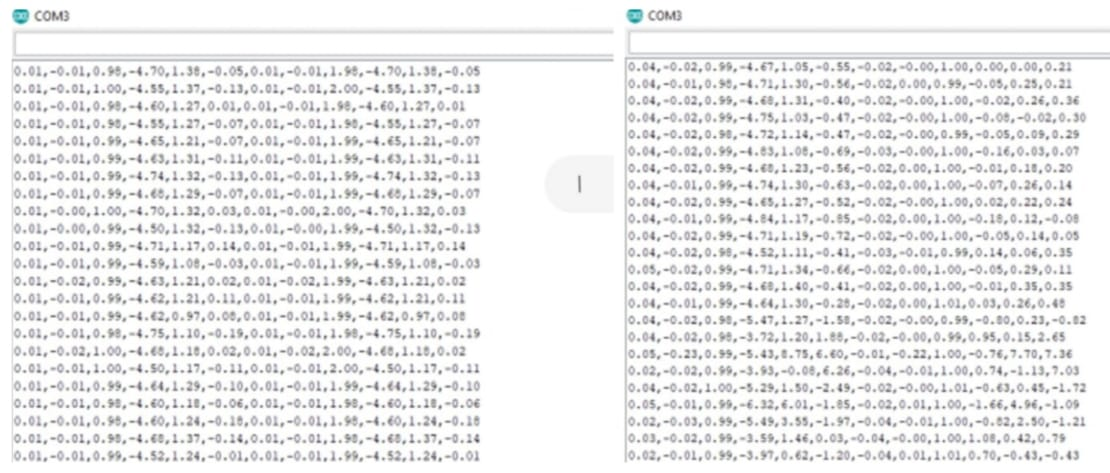
\includegraphics[width=8cm]{Figuras/calibrados_sincalibrar.jpg}
\caption{Datos sin calibrar/ Datos calibrados}
\label{fig:calibrados_sincalibrar}
\end{figure}

A continuación se podrá realizar el análisis visual de la gráfica (Fig.5) y el comportamiento de los datos sin calibrar del acelerómetro donde se observa claramente lo mencionado anteriormente que los valores de los ejes X y Y se encuentran un poco desviados de su punto de precisión 0 y igual para la linea delineada de verde que nos simboliza el eje z vemos como principio se encuentra muy cercana a 1 y finalizando ya se encuentra mas alejada del setpoint mencionado.
\begin{figure}[htbp]
\centering
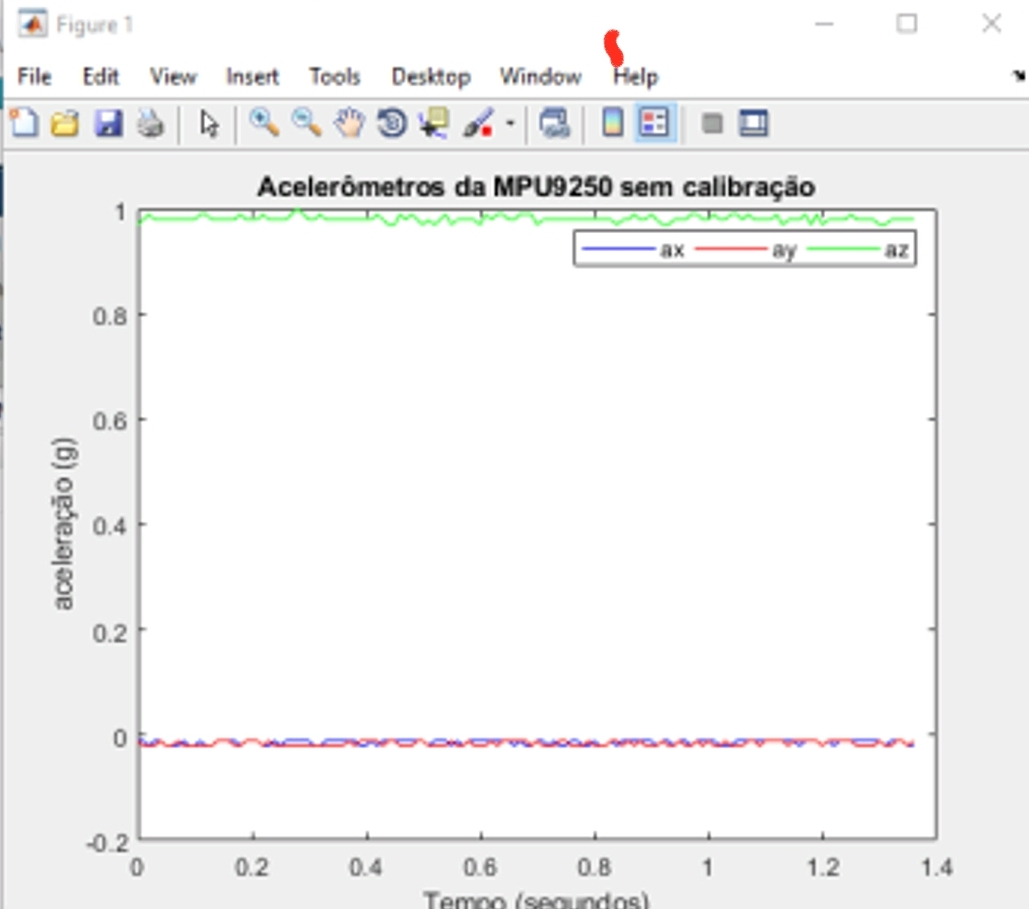
\includegraphics[width=7cm]{Figuras/acelerometro sin calibrar.jpeg}
\caption{Grafica de acelerometro sin calibrar}
\label{fig:acelerometro sin calibrar}
\end{figure}\\
Luego del proceso de ajuste o calibracionde las variables se ve claramente un mejor comportamiento de las variables X y Y practimente en 0 y la variable Z completamente en valores de 1 en la Fig.6.
\begin{figure}[htbp]
\centering
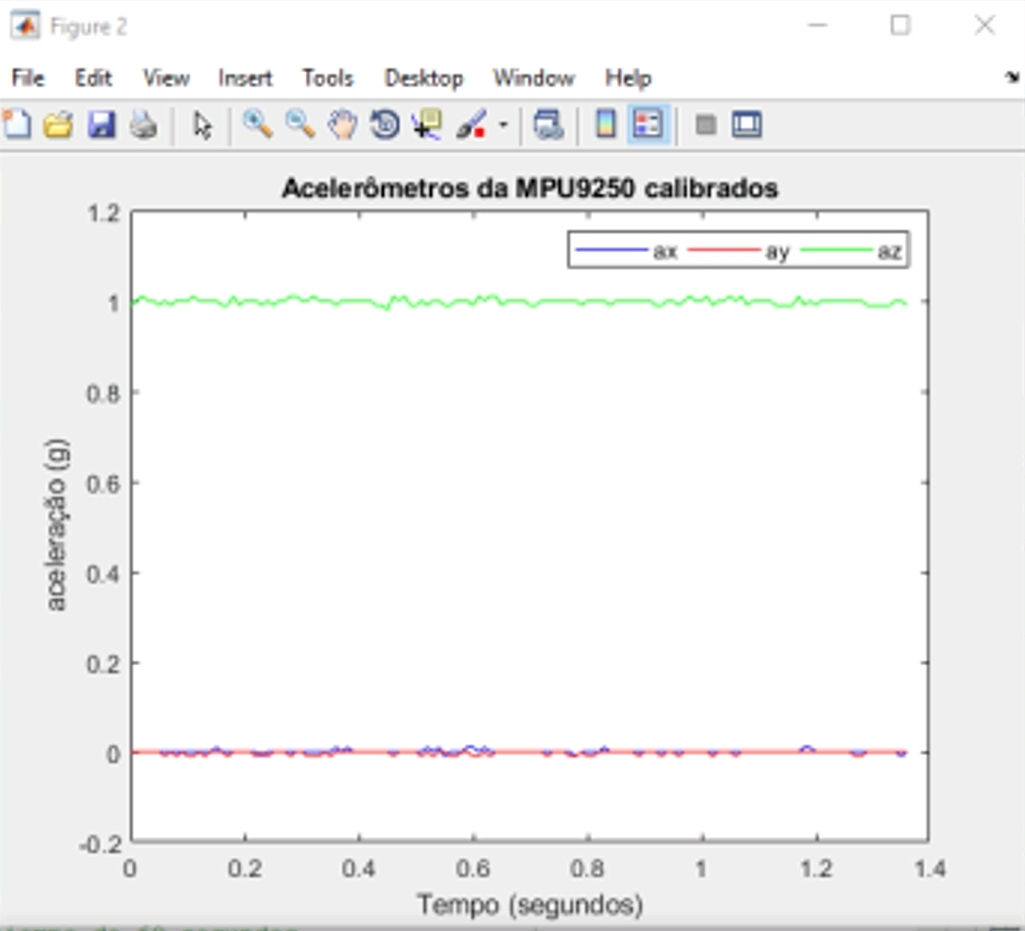
\includegraphics[width=7cm]{Figuras/acelerometro calibrado.jpeg}
\caption{Gráfica de acelerómetro calibrado}
\label{fig:acelerometro calibrado}
\end{figure}\\
En la Fig.7 se observa que la velocidad angular a las que responde el sensor se encuentran completamente desviadas en todos sus ejes pero el que mas requeria de calibracion era la variable del eje x que se encontraba cerca a los -5 m/s representado por una linea azul.\\
\begin{figure}[htbp]
\centering
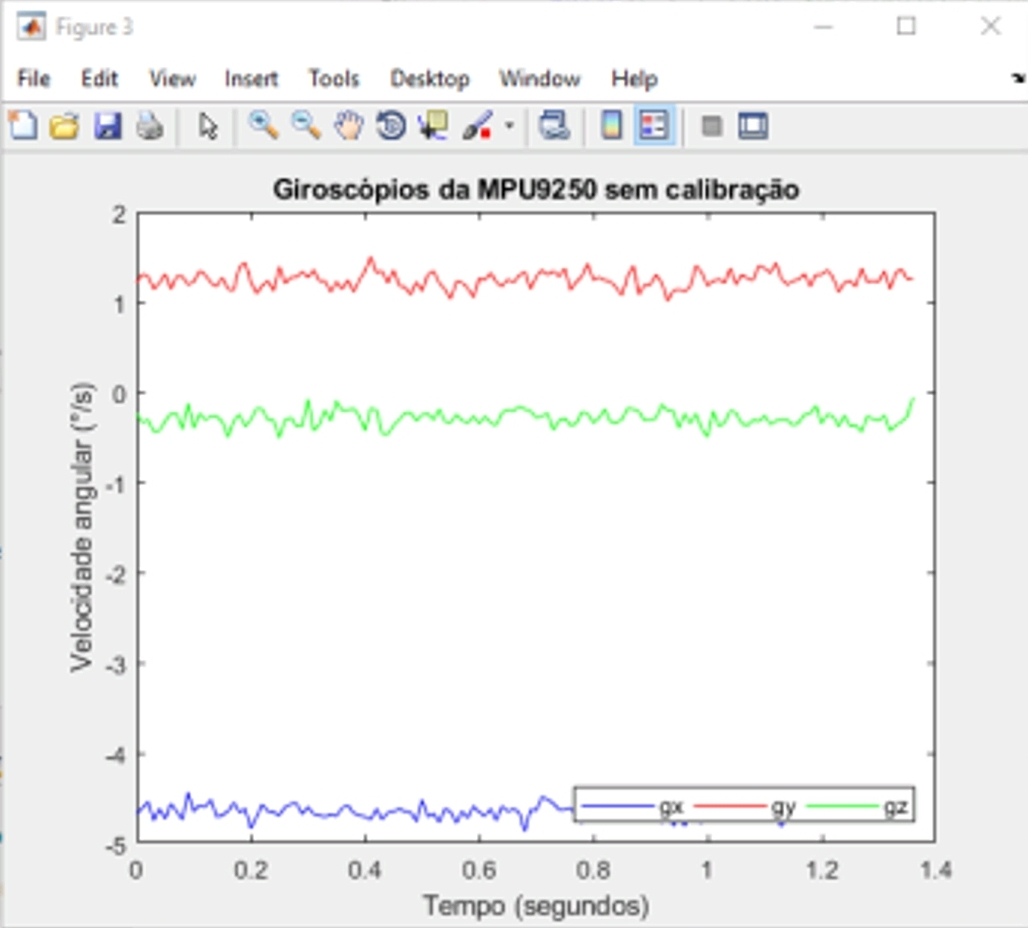
\includegraphics[width=7cm]{Figuras/giroscopio sin calibrar.jpeg}
\caption{Gráfica del giroscopio sin calibrar}
\label{fig:giroscopio sin calibrar}
\end{figure}
Luego de realizar la calibración pertinente igualmente como sucedió con el acelerómetro obtenemos en la gráfica de la Fig.8 una respuesta totalmente precisa ya que los valores se encuentran muy cercanos a 0 como se veía en los datos del visualizador
\begin{figure}[htbp]
\centering
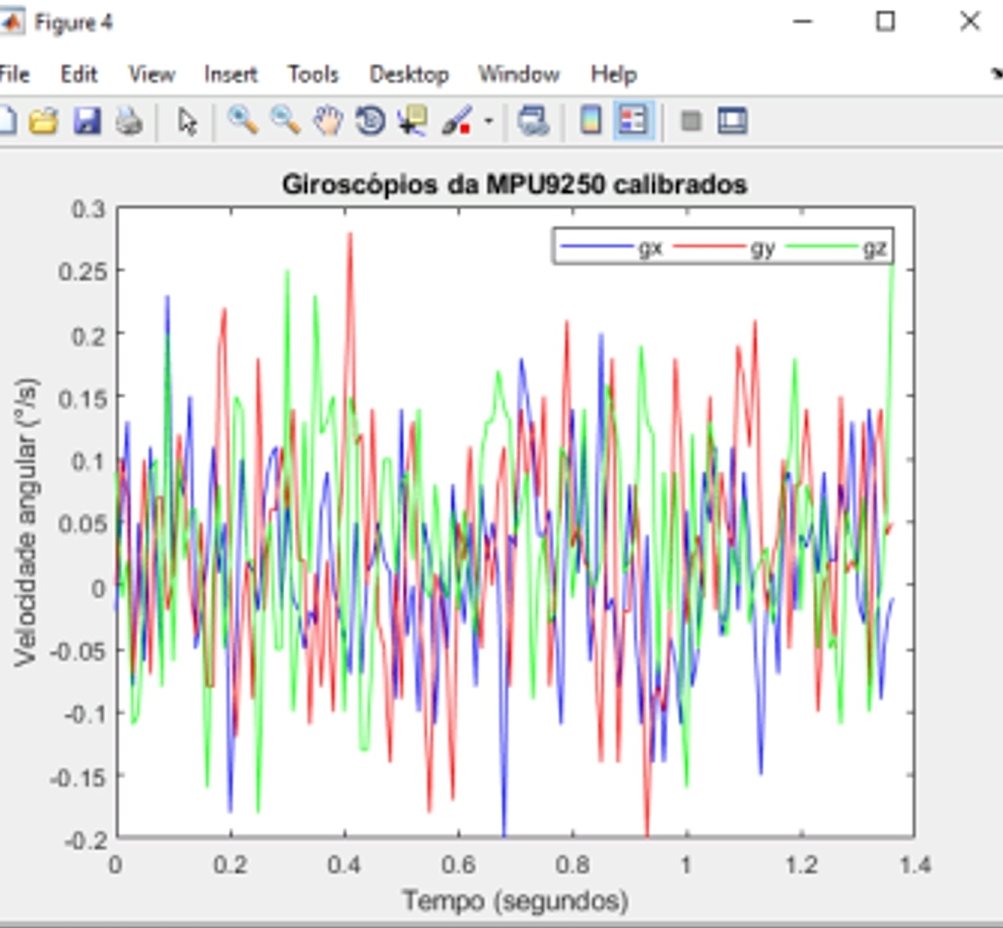
\includegraphics[width=7cm]{Figuras/giroscopio calibrado.jpeg}
\caption{Gráfica del giroscopio calibrado}
\label{fig:giroscopio calibrado}
\end{figure}
\section{Conexion VNC} \label{sec:VNC}
Para realizar las conexion VNC de la raspberry, se logra conectando el dispositivo desde donde se va a trabajar en este caso el PC a una red wifi a la que se debera conectar tambien la tarjeta, para ello deberemos disponer de 3 perifericos como lo son una pantalla, un teclado y un mouse que se utilizaran para en primer lugar para conectar la pi3 a la red de internet, luego procedemos a descargar el programa VNC en esta(raspberry) introduciremos posteriormente ifconfig para visualizar la IP y esta direccion la introduciremos en el programa VNC descargado con anterioridad en el PC utilizando el protocolo de comunicacion IP para realizar un control remoto de la raspberry pi3
